\documentclass[a4paper]{jpconf}
\bibliographystyle{iopart-num}
\usepackage{amsmath}
\usepackage{citesort}
\usepackage{subfigure}
\usepackage{graphicx}
\graphicspath{{fig/}}
\usepackage{ifpdf}
\ifpdf\usepackage{epstopdf}\fi
\usepackage[export]{adjustbox}

%----------------------------------------------------- 
%\usepackage{soul,ulem,color,xspace,bm}
% Andrei's commands
% Suggest to remove
%\newcommand{\asrm}[1]{{\color{magenta}\sout{#1}}}
% Suggest to insert
%\newcommand{\as}[1]{\color{cyan}#1\xspace\color{black}}
% Suggest to replace
%\newcommand{\asrp}[2]{\asrm{#1} \as{#2}}
% Comment
%\newcommand{\ascm}[1]{{\color{green}\;AS: #1}}
%------------------------------------------------------

\begin{document}
\title{Electron and ion acceleration by relativistic shocks: particle-in-cell simulations}

\author{V I Romansky$^{1,2}$, A M Bykov$^{1,3}$ and S M Osipov$^1$}

\address{$^1$ Ioffe Institute, 26 Politekhnicheskaya st., St. Petersburg 194021, Russia}
\address{$^2$
	Sternberg Astronomical Institute, Moscow State University
	Universitetsky pr., 13, Moscow 119234, Russia}
\address{$^3$ Peter the Great St.~Petersburg Polytechnic University, 29 Politekhnicheskaya st., St. Petersburg 195251, Russia}

\ead{romanskyvadim@gmail.com}

\begin{abstract}
	The problem of particle acceleration by collisionless astrophysical shocks is of fundamental importance for the cosmic ray origin problem and  for the high energy astrophysics as a whole. Fast magnetohydrodynamical shocks produced by relativistic jets are considered as very likely sites of cosmic ray acceleration.
	While cosmic ray acceleration by both non-relativistic and ultra relativistic shocks was studied in some details, the shocks of moderate Lorentz factors have attracted much less attention so far, while they are important for modeling gamma-ray burst afterglows and a number of other interesting objects. In this paper we present simulations of relativistic shock waves in electron-proton plasmas obtained with an implicit particle-in-cell code for the initial study the particle injection efficiencies.
\end{abstract}
\section{Introduction}
One of the possible sources of high-energy cosmic rays (CRs) are shock waves in astrophysical collisionless plasmas which are believed to accelerate particles via  the diffusive shock acceleration (DSA) mechanism, see, e. g. \cite{Bell1978}, \cite{Blandford1978}. The particle acceleration in the vicinity of shock front is a sophisticated and nonlinear problem, because the CRs strongly influence on the structure of the shock. Their pressure is comparable with the pressure of background plasma and significantly modifies the shock front (see, e.g., \cite{Bykov2014}). 
Also the instabilities in the anisotropic plasma can result to a strong magnetic field amplification. The spectra of synchrotron emission observed from supernova remnants (SNRs) indicate that the magnetic field in their shells is about 100 times stronger than the interstellar field (see, e.g., \cite{Berezhko2003},\cite{Uchiyama2007}). 
One of the most powerful methods to explore the processes in collisionless plasma is particle-in-cell (PIC) simulation.

\section{Shock wave simulation}
We studied the evolution of moderately relativistic shocks and spectra of accelerated particles. We chose relativistic shocks with a relatively low Lorentz factor ($\gamma=1.5$) because the maximum energy of the produced CRs cosmic rays increases with the shock Lorentz factor, while the efficiency of acceleration decreases, 
because it becomes more difficult for particle to cross fast moving front
%
\cite{Ellison2013}. So we assumed that an intermediate case of moderately relativistic shocks would provide the most efficient acceleration.

To perform the simulations we developed the implicit PIC code \cite{Romansky2016}, based on the scheme suggested by Lapenta et al.~\cite{Lapenta2006} and improved for the relativistic case by Noguchi et al.\cite{Noguchi2007}.
The code is fully three-dimensional and parallelized with MPI technology. The electric field divergence is corrected
after every several time steps and 
the shortwave harmonics Fourier filtering is applied
to suppress the numerical Cherenkov instability and improve energy conservation.

In the modeling setup the homogeneous plasma flows into the simulation box through its right boundary
and collides with the reflecting superconducting wall at the left boundary thus launching a shock wave. This  is a common way to initialize a shock, because an initialization using the Rankine-Hugoniot conditions does not take into account the microscopic distribution, and a shock, created in such a way, would probably fall apart into several discontinuities.

\begin{figure}[h!]
	\centering
	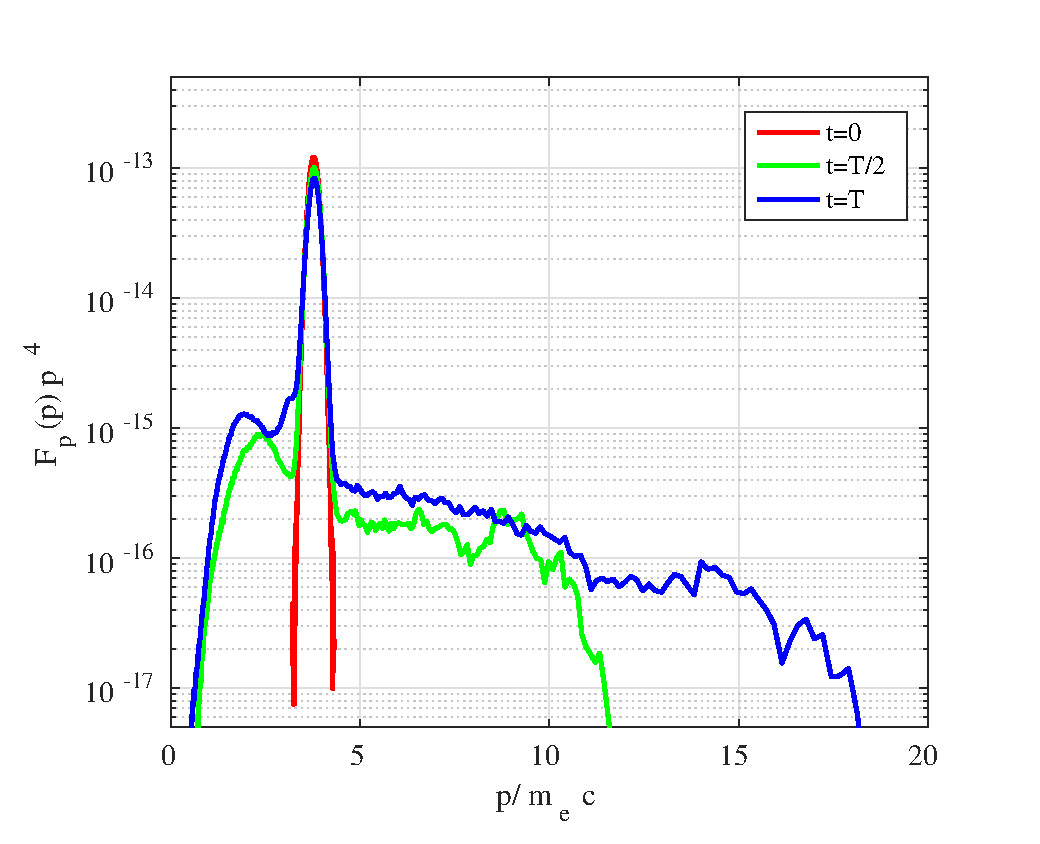
\includegraphics[width=1.0\textwidth]{fig/protons.eps} 
	\caption{Distribution of protons in a relativistic shock wave with Lorentz factor 1.5 at various inclination angle $\theta$.}
	\label{protons}
\end{figure} 

The simulations are one-dimensional and have the following parameters of the initial flow: Lorentz factor $\gamma = 1.5$, the number densities $n_e = 10^{-4} \rm{cm}^{-3}$, $n_p = 10^{-4} \rm{cm}^{-3}$ , the temperature, $T_e = T_p = 5\cdot10^8 \rm{K}$, the magnetic field $B = 10^{-4} \rm{G}$, the full size of the box $L = 2\cdot10^{12} \rm{cm}$, the number of cells $N=2\cdot10^4$. The electron mass $m_e$ is increase by $100$ times to enlarge electron scales of  the plasma, it is common approach in PIC simulations see e.g. {\cite{Sironi2011}} to reduce required computational recources. The full time of simulation is $T = 5000 {\omega_p}^{-1}$, where $\omega_p$ is electron plasma frequency.These values allow one to define the dimensionless parameter magnetization $\sigma = B^2/4\pi\gamma (n_p m_p + n_e m_e) c^2 = 0.003$. Inclination angle $\theta$ is the angle between the flow velocity and the magnetic field. We present results for the particle spectrum in several simulations at various $\theta$. Stable shocks formed in all simulations and the total energy of the system conserved to better than $3\%$, which indicates that the code provides a correct model of the shock waves. 


\begin{figure}[h!]
	\centering
	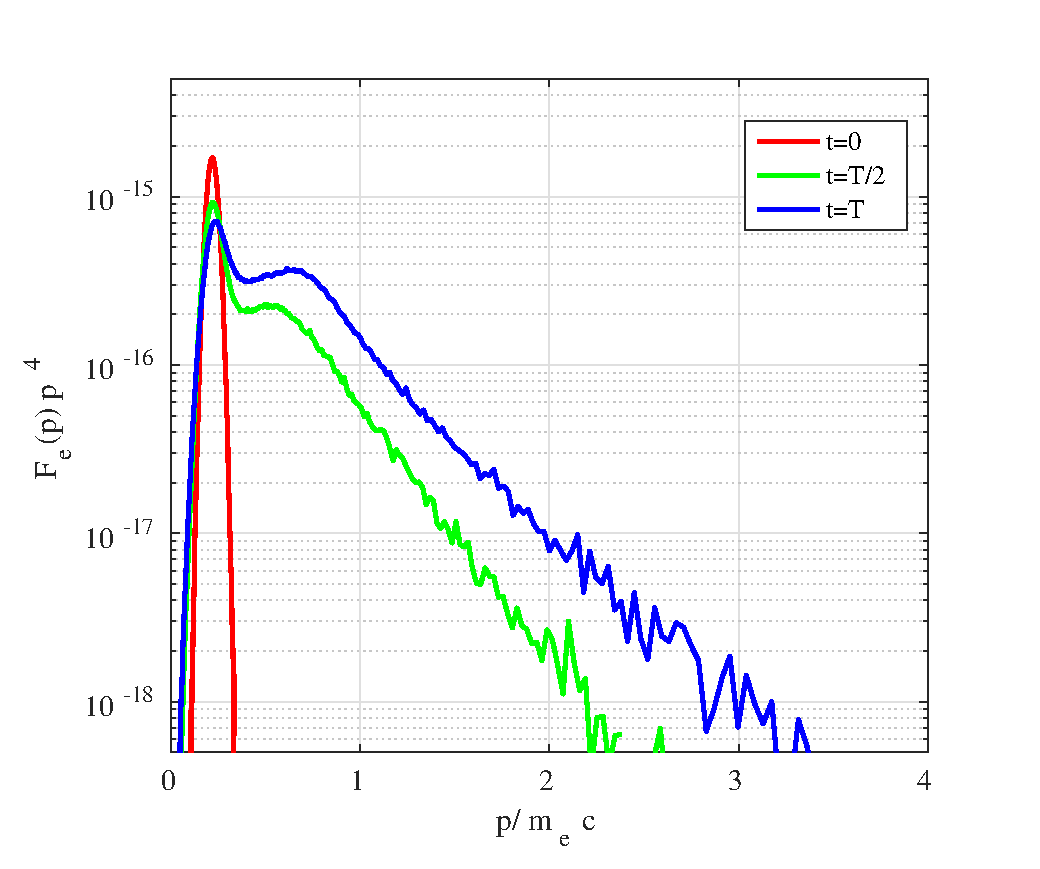
\includegraphics[width=1.0\textwidth]{fig/electrons.eps} 
	\caption{Distribution of electrons in a relativistic shock wave with Lorentz factor 1.5 at various inclination angle $\theta$.}
	\label{electrons}
\end{figure}

One can see in Figures \ref{protons} and \ref{electrons} the particle spectra for various inclination angles $\theta$. The spectra consist of three parts - the narrow peak of cold but fast moving initial flow, approximated by Maxwell distribution, shifted on the initial momentum, the wide peak of hot downstream, approximated by Maxwell-J{\"u}ttner distribution, and the non-thermal accelerated component. The small-scale oscilations of spectra are produced by numerical errors and should not be taken into account. Figures show that the spectrum of accelerated particles strongly depends on he inclination angle $\theta$. If $\theta$ is less than the critical value, defined by the equation $c\cdot \cos(\theta_{crit})=v_{shock}$, where all values are measured in the upstream rest frame, particles can escape from the front and cross it several times to gain more energy (see, e.g., \cite{Pelletier2017}), if $\theta$ is greater, shock becomes superluminal - particles need to move along the field lines faster than light to escape from the front, and acceleration is suppressed. It is difficult to evaluate the critical angle \textit{a priori}, because the compression relation of the shock which will be created in the simulation is unknown. However the estimate for the case of a strong wave (the compression relation equals $4$) provides $\theta_{crit}=45^{\circ}$ in the downstream frame, which is consistent with the results of our simulations.

Also, one can see that for the angles less then the critical one, concentrations of accelerated particles are higher and extend to higher enegies for larger $\theta$. The spectrum of non-thermal component is about 10 times higher for the protons than for the electrons at the same energy. It is consistent with other PIC simulations of the shock waves {\cite{Sironi2011}}.

These results show some interesting effects for angles close to the critical value (black and yellow lines)- the electrons are still accelerating while the protons are not. It can be interpreted as electrons accelerate in the short-wavelength turbulence of the shock precursor. Due to the small gyroradii of the electrons in initial flow, the short-wavelength turbulence scatter them more efficiently than protons. However, further research is necessary to study this phenomenon in detail.


\section{Conclusions}
In this paper we presented results of the PIC simulations of particle acceleration by moderately relativistic shock waves in space plasmas. Simulations show, that injection of particles into the acceleration process strongly depends on the angle between the flow bulk velocity and the magnetic field. The injection efficiency as a function of the inclination angle has been studied. Injection of protons is more efficient than that of electrons for the inclination angles below the critical angle where the transition to the superluminal shock regime occurs. On  another hand the electron acceleration is more efficient in shocks with the inclination angles close to the critical angle.
\ack
V I Romansky acknowledges support from RSF grant 16-12-10519.
The numerical results presented here were obtained using computational resources of Peter the Great Saint-Petersburg Polytechnic University Supercomputing Center (http://www.scc.spbstu.ru). 

\section*{References}
\begin{thebibliography}{20}
	\bibitem{Bell1978} Bell A R 1978 \textit{MNRAS} \textbf{182} 147
	\bibitem{Blandford1978} Blandford R D and Ostriker J P 1978 \textit{ApJ} \textbf{221} L29 
	\bibitem{Bykov2014} Bykov A M, Ellison D C, Osipov S M and Vladimirov A E 2014 \textit{ApJ} \textbf{789} Issue 2, 137
	\bibitem{Berezhko2003} Berezhko E G, Ksenofontov L T and V{\"o}lk H J  2003 \textit{A}{\&}\textit{A} \textbf{412} L11
	\bibitem{Uchiyama2007} Uchiyama Y, Aharonian F A, Tanaka T, Takahashi T and Maeda Y 2007 \textit{Nature} \textbf{449} 576
	\bibitem{Romansky2016} Romansky V I, Bykov A M, Osipov S M and Gladilin P E 2017 \textit{Journal of Physics: CS} \textbf{929} id 012014 
	\bibitem{Lapenta2006} Lapenta G, Brackbill J U and Ricci P 2006 \textit{Phys. Plasmas} \textbf{13} 055904
	\bibitem{Noguchi2007} Noguchi K, Tronci C, Zuccaro G and Lapenta G 2007 \textit{Phys. Plasmas} \textbf{14} 042308
	\bibitem{Ellison2013} Ellison D C, Warren D C and Bykov A M 2013 \textit{ApJ} \textbf{776} Issue 1, 46
	\bibitem{Pelletier2017} Pelletier G, Bykov A M, Ellison D C and Lemoine M 2017 \textit{Space Science Reviews} \textbf{207} Issue 1-4, pp. 319-360
	\bibitem{Sironi2011} Sironi L and Spitkovsky A 2011 \textit{ApJ} \textbf{741} Issue 1, 39
\end{thebibliography}
\end{document}